\section{Levantando o programa}\label{program}

Inicialmente, é importante frisar que o kit do Arduíno nada mais é que uma camada de abstração criada acima do microcontrolador AVR. Desta forma, podemos programar nos kits do Arduíno de duas formas sob o sistema Linux:

\subsection{Shield Comum}\label{noob}

A forma mais simples de utilizar um kit do Arduíno é utilizando a própria IDE oferecida para o kit. A sua instalação é bem simples e fácil de ser feita. Basta entrar com o seguinte comando no terminal:


\begin{lstlisting}[style=Bash,numbers=none]
user@DESKTOP: sudo apt-get install arduino
\end{lstlisting}

Desta forma, podemos acessar a IDE do Arduíno, que pode ser observada na figura \ref{arduino_ide} e escrever o programa tranquilamente, utilizando apenas as funções $loop$ e $setup$.

\end{multicols}
\begin{figure}[H]
\begin{center}
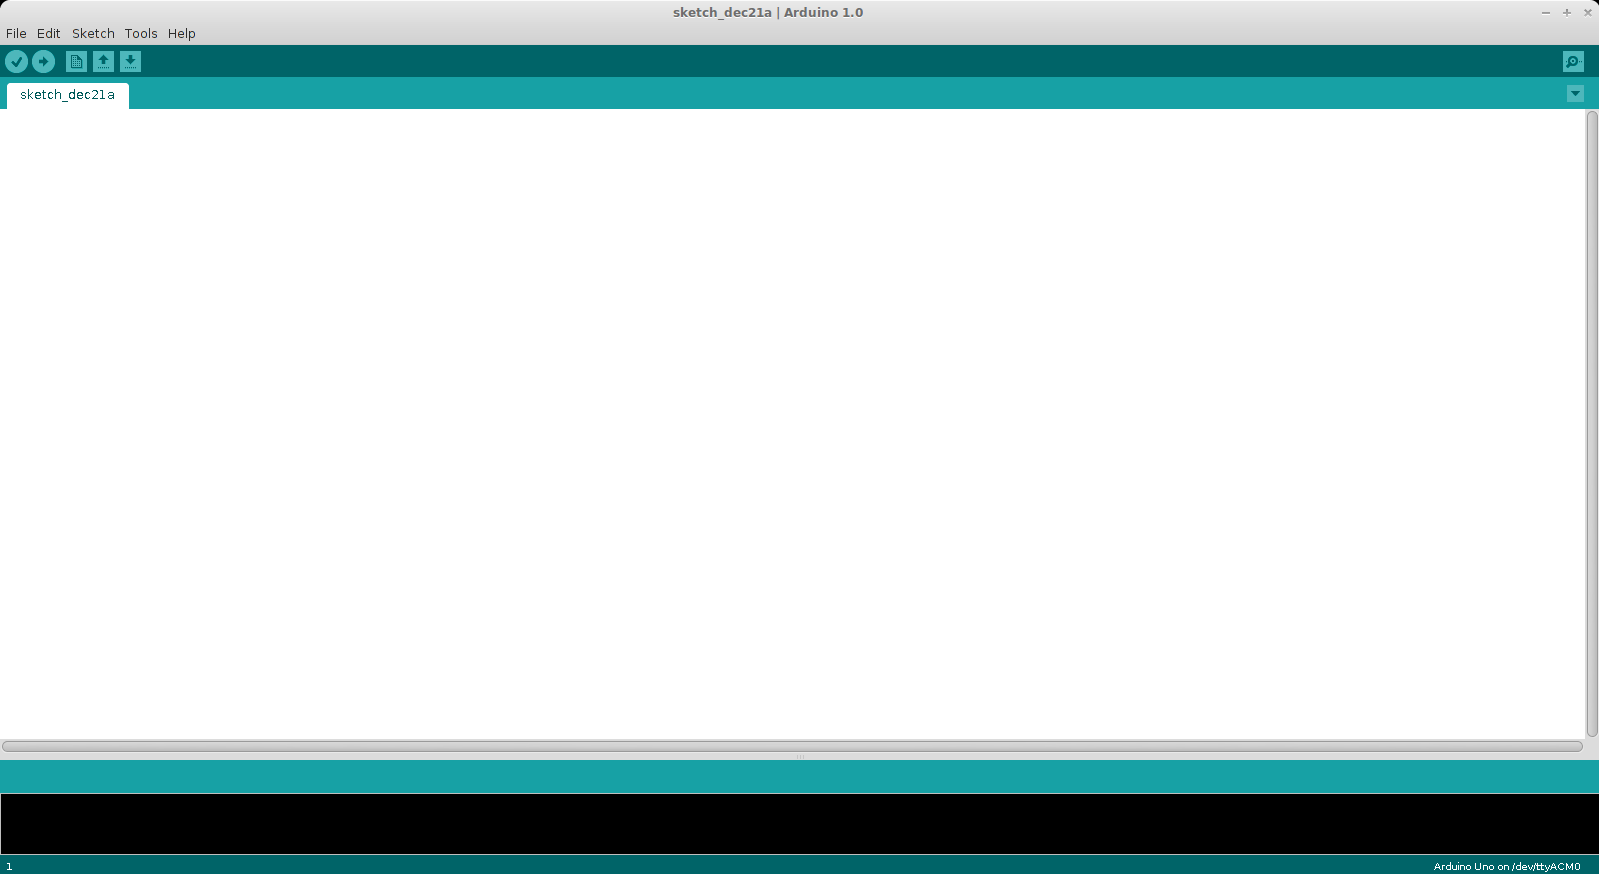
\includegraphics[scale=0.25,angle=0,keepaspectratio=true]{./fts/arduino_ide.png}
\end{center}
\caption{IDE do Arduino}
\label{arduino_ide}
\end{figure}
\begin{multicols}{2}    % 2 columns

\subsection{Utilizando o Eclipse para o Arduino}\label{eclipse}

Porém há alguns grandes inconvenientes ao utilizar a IDE do Arduino.

\begin{itemize}
	\item Todas as bibliotecas serão compiladas sempre
	\item O editor de texto deixa muito a desejar
	\item Não há uma função de auto-completar para facilitar o uso das funções já criadas
\end{itemize}

Desta forma, uma opção interessante é utilizar o Eclipse para programar o Arduíno. Isso requer alguns conceitos mais avançados de programação que não serão descritos neste relatório, que são eles:

\begin{itemize}
	\item Criação de uma biblioteca estática com os arquivos em $/usr/shared/arduino$.
	\item Inclusão do diretório $/usr/shared/arduino$ nas dependências da compilação.
	\item Configuração da compilação com as flags $-Os$,$-O3$ e $-g$.
	\item Instalação do plugin de AVR no Eclipse e do AvrDude
\end{itemize}

Outro fator interessante de se usar o Eclipse é a necessidade de fazer uma função $main$, já que esta é descartada pela IDE do Arduíno. Abaixo segue um exemplo de como a função $main$ poderia ser escrita para ter um funcionamento semelhante ao da IDE do Arduíno, facilitando assim a compatibilidade entre os códigos.

%\end{multicols}
\begin{lstlisting}[basicstyle=\ttfamily,numbers=none,caption={[Exemplo da função main()]Código de exemplo da função main()}]

#include <Arduino.h>

int main(void)
{

	init();
	setup();

	while(true) 
		loop();

	return 0;
}
\end{lstlisting}
%\begin{multicols}{2}    % 2 columns

Observe que este código mantem toda a estrutura básica do Arduíno, assim como a inclusão do header $Arduino.h$, necessário para a inclusão das rotinas básicas do Arduíno, assim como sua configuração.

\subsection{Criação do Código}\label{making}

Com o ambiente de trabalho já configurado, o próximo passo é levantar o programa que funcione de acordo com o diagrama, apresentado na figura \ref{flux_micro}.

\begin{figure}[H]
\begin{center}
\begin{tikzpicture}[node distance = 2cm]
	\tiny\ttfamily
	%-- Estados
	\node [cloud] (init) at(0,0) {Inicio};
	\node [estado] (E1) at(2,0) {Inicializa\\ UART e ADC};
	\node [estado] (E2) at(4,0) {Captura ADC};
	\node [estado] (E3) at(4,-2) {Escreve ADC na UART};
	%-- Setas
	\path (init) edge [line] (E1);
	\path (E1) edge [line] (E2);
	\path (E2) edge [bend right,->] (E3);
	\path (E3) edge [bend right,->] (E2);
\end{tikzpicture}
%\\\hypertarget{diagrama}{Fluxograma do microcontrolador}
\end{center}
\caption{Fluxograma do microcontrolador}
\label{flux_micro}
\end{figure}

Como descrito no diagrama, é necessário inicializar tanto a UART (Comunicação Serial) quanto o ADC (Conversor Analógico-Digital) antes de prender o microcontrolador no laço infinito de captura e exportação dos valores do ADC. Seguindo o contexto de manter a máxima semelhança com o modelo proposto de programação no Arduino, inicializaremos a UART e o ADC na função $setup$ da seguinte forma:

\begin{lstlisting}[basicstyle=\ttfamily,numbers=none,caption={[setup()]Código da função setup()}]

void setup()
{
	Serial.begin(9600);
	analogReference(EXTERNAL);
}

\end{lstlisting}

Observe que a UART é inicializada com rate de 9600, enquanto o conversor é configurado para usar a referencia de tensão externa. A velocidade de 9600 é uma faixa de velocidade bem comum em comunicações seriais. Já a referencia externa é necessária devido ao circuito que foi proposto na sessão \ref{cirt_final_sec}, onde a figura \ref{final} apresenta uma tensão de referencia.

Com o chip já configurado, o próximo passo é configurar a função $loo$ para que o processo de captura do valor do ADC e impressão deste valor seja mantido enquanto o chip estiver alimentado.



\begin{lstlisting}[basicstyle=\ttfamily,numbers=none,caption={[setup()]Código da função setup()}]

void loop()
{
static int i=0;
char buf[20];

	sprintf(buf,"%d %d\n",i++,analogRead(0) );
	Serial.print(buf);
}
\end{lstlisting}

Desta forma, os valores serão impressos na porta serial com a formatação \textit{"x y"}, estando assim prontos para serem plotados no GNUPLOT. No apêndice \ref{src} pode-se observar na integra este código no Listing
\ref{main}, onde haverá a inclusão de alguns headers e alguns tempos no decorrer do programa para garantir uma maior estabilidade do código.






